\documentclass[10pt]{beamer}

% Package
\usepackage{graphicx}
\usepackage{tcolorbox}
\usepackage{listings}

% Theme
\usetheme{Warsaw}
\usecolortheme{beaver}

% Main & Info
\title[Angular]
{Module Angular}
\subtitle{Parti 1}
\author[Maxime Tournier]
{Maxime Tournier}
\date[21/08/2023]

% Start
\begin{document}

	\frame{\titlepage}

	\begin{frame}
		\frametitle{Sommaire}

		1. {Présentation} \newline
		2. {Histoire} \newline
		3. {Démarrage Angular} \newline
		4. {TypeScript} \newline
		4. {Premier pas sur Angular} \newline
		5. {Composants} \newline
		6. {Template} \newline
		7. {Route} \newline

	\end{frame}

%%%%%%%% Présentation

	\begin{frame}
		\frametitle{Présentation}
	
		Angular est un \alert{FrameWork}

		\begin{block}{Traduction}
			Framework = Cadre de travail
		\end{block}

		En tant que développeur on fait souvent la meme chose \newline \newline
		Exemple: \newline Valider les formulaires | Gerez la navigation | traiter les erreurs
		\newline \newline
		Et pour regler ce problème au lieu d'allez recupere les fonction d'autre projet on à créer les framework
		\newline \newline
		Avantage : Tout le monde travaille sur les même fonction
		
	\end{frame}

	\begin{frame}
		\frametitle{Présentation}

		Pour comprendre le fonctionnement d'angular
		\newline \newline
		Il faut comprendre le web aujourd'hui
		\newline \newline
		Site Web / Application Web
		\newline \newline
		Il s'agit bien de deux chose différente

	\end{frame}

	\begin{frame}
		\frametitle{Présentation}

		Avant ça comment ça marche :

			
\includegraphics[width=2cm]{assets/page}\newline
			- Fichier client (CSS, HTML, JS)

			
\includegraphics[width=2cm]{assets/server}\newline
			- Fichier serveur (php, java) (ici qu'on fait des requetes sql)

	\end{frame}

	\begin{frame}
		\frametitle{Présentation}

		Et donc un site web fonctionne comme ça :
		\newline \newline

		\centering
		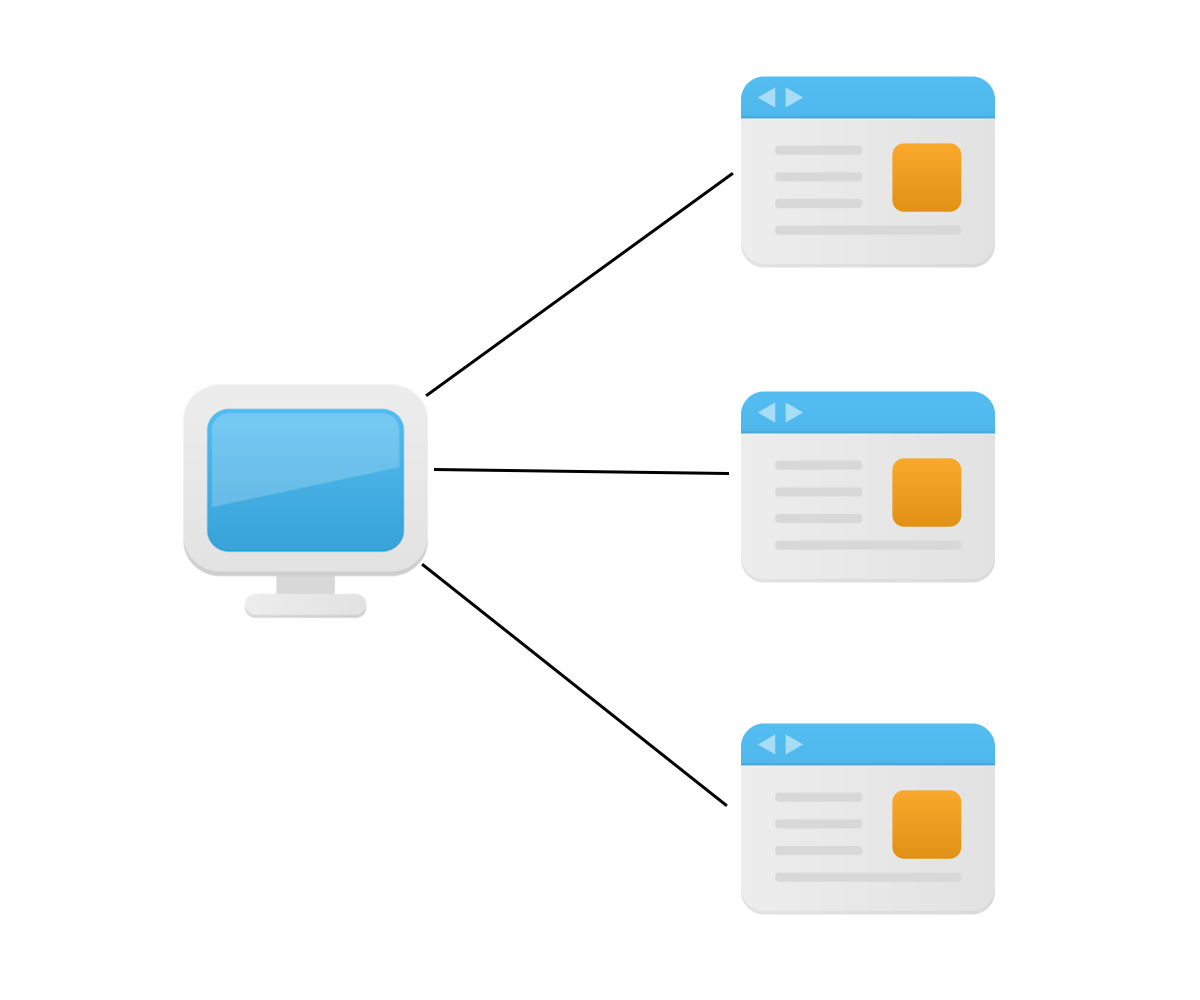
\includegraphics[width=6cm]{assets/siteweb}\newline

	\end{frame}

	\begin{frame}
		\frametitle{Présentation}

		Et une application web marche comme ça:
		\newline \newline

		\centering
		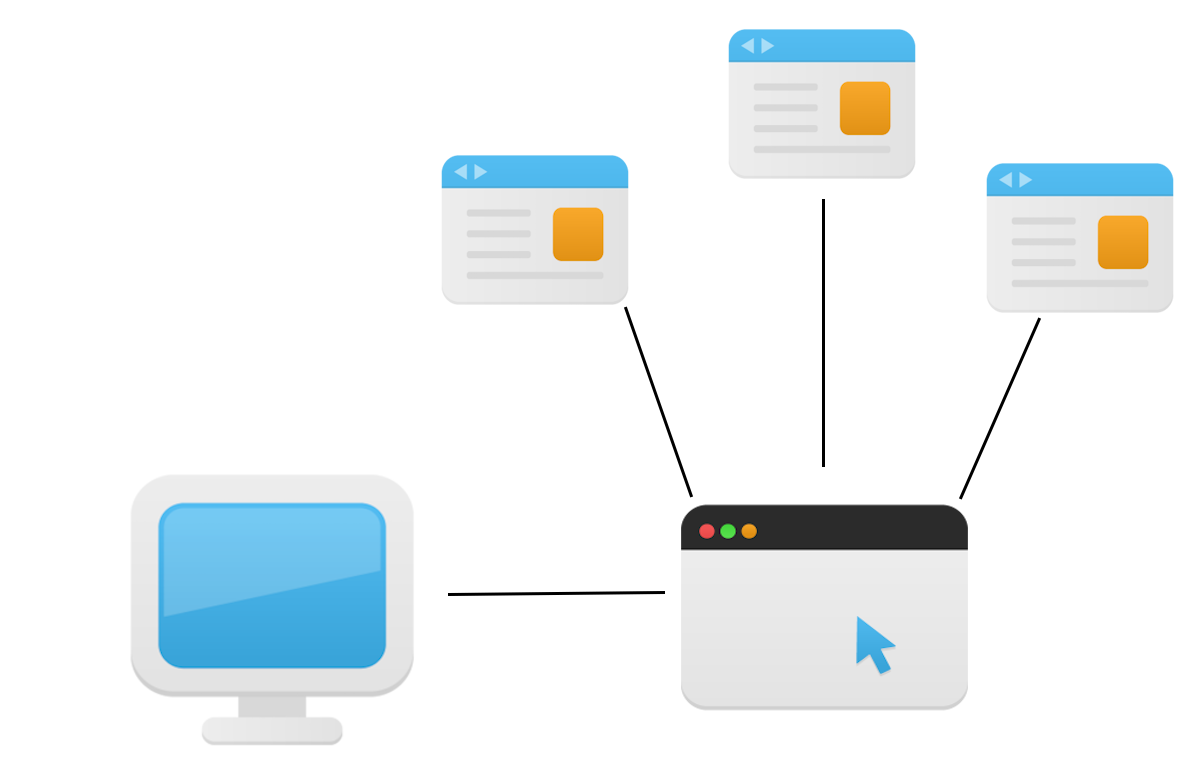
\includegraphics[width=8cm]{assets/appweb}\newline

	\end{frame}

	\begin{frame}
		\frametitle{Présentation}

		Resumé :
		\newline \newline
		le client doit faire une requête au serveur a chaque fois dans un site web \newline \newline
		alors que dans une application web, nous allons deleguer le travaille a JavaScript qui vas désactivé ou activé une parti du code html/css
		\newline \newline
		\begin{block}{Information}
			Cette méthode s'appel SPA (Single Page Application)
		\end{block}
	\end{frame}

%%%%%%%% Histoire

	\begin{frame}
		\frametitle{Histoire}

		AngularJS n'est pas egal a Angular \newline \newline

		AngularJS à été créer par Google \newline \newline

		AngularJS avait comme architecture MVC \newline \newline

		AngularJS n'est plus maintenu depuis 2018 \newline \newline

		\begin{block}{MVC}
			Module Vue Controlleur (Comme Symfony)
		\end{block}

	\end{frame}

	\begin{frame}
		\frametitle{Histoire}

		Angular est un framework orienté composant \newline \newline

		Nous allons codé une multitude de petit composant qui formeront une application \newline \newline

		Un composant est une parti du site qui fonctionne de manière autonome sur une applicaiton

	\end{frame}

	\begin{frame}
		\frametitle{Histoire}

		Angular est il difficiel à apprendre ? : \newline \newline

		Angular à une réputation de framework difficile \newline \newline

		Car Angular est basé sur TypeScript un languge basé sur Javascript qui permet de Typé vos variable \newline \newline

		Angular est basé sur la version de Javascript ES6

	\end{frame}

	\begin{frame}
		\frametitle{Information}
		\centering
		Regarder la documentation
		S'IL VOUS PLAIT

		Angular.io

	\end{frame}

%%%%%%%% Demarrage Angular

	\begin{frame}
		\frametitle{Démarrage Angular}

		1. Installer un environnement de developpement \newline
		2. Genere un socle angular (Grâce à Angular-CLI) \newline
		3. Nous allons jouer avec le composant racine =)
		\newline \newline
		\begin{block}{Information}
			un composont c’est comme une parti de l’application web. Mais il y a un premier composant a l'origine de tout, que nous appelons le composant racine
		\end{block}

	\end{frame}

	\begin{frame}
		\frametitle{Démarrage Angular}

		Ce qu'on a besoin : \newline \newline

		D'abors on vas avoir besoin du moteur javascript (NodeJS) et d'un gestionnaire de packet (NPM) \newline \newline

		D'un Editeur de code TypeScript \newline \newline

		Un outil qu'on appel Angular CLI (Qui vas nous permet de gérez notre projet Angular)

	\end{frame}

	\begin{frame}
		\frametitle{NodeJS et NPM}

		NodeJS et NPM sont utiliser pour la majorité des projet JavaScript moderne \newline \newline

		NodeJS permet d’excute du code JS coté serveur \newline \newline

		NPM permet de gere les dépence de paquet de javascript (angular est un paquet) \newline \newline

		NodeJS integre par defaut NPM

	\end{frame}

	\begin{frame}
		\frametitle{NodeJS et NPM}

		Pour installer NodeJS (et donc aussi NPM) \newline \newline

		il vous suffit d'installer sur le site officiel https://nodejs.org/fr \newline \newline

		\begin{block}{Information}
			Prenez la version LTS
		\end{block}

	\end{frame}

	\begin{frame}
		\frametitle{IDE}

		On vas avoir besoin d'un IDE \newline \newline

		Un IDE est un environnement de developpement (Editeur de code amélioré) \newline \newline

		- Visual Studio Code : Recommander par Mircorsoft (Gratuit) \newline
		- WebStorm : Beaucoup plus puissant et recommander par Google, de la suite JetBrain (Payant) \newline  \newline

		Choissier celui que vous préfèrer ou que vous êtes le plus a l'aise  \newline \newline

		\begin{block}{Information}
			La suite JetBrain (WebStorm) est gratuit pendant tout au long de votre formation, inscription sur leurs site internet
		\end{block}

	\end{frame}

	\begin{frame}
		\frametitle{Terminal}

		Pour votre terminal : \newline \newline

		Souvent il peut avoir des problème avec le terminal Windows \newline \newline

		Essayer de toujours d'utiliser PowerShell \newline \newline

	\end{frame}

	\begin{frame}
		\frametitle{Démarrage Angular}

		Activité :  \newline \newline

		- Installer NodeJS et NPM sur le site officiel (https://nodejs.org/fr)
		Prenez la version LTS pour NodeJS  \newline \newline

		- Installer un IDE : Visual Studio Code ou WebStorm  \newline \newline

		Pour tester si NodeJS et NPM son bien installer, Ouvrez un terminal  \newline
		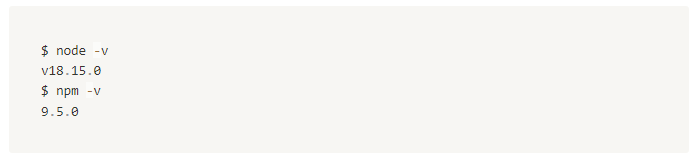
\includegraphics[width=10cm]{assets/npminstall}\newline

	\end{frame}

%%%%%%%% TypeScript

	\begin{frame}
		\frametitle{TypeScript}

		TypeScript est une surcouche de JavaScript  \newline \newline

		TypeScript est developed par Microsoft depuis 2012  \newline \newline

		TypeScript support les dernier version de JS ES6

	\end{frame}

	\begin{frame}
		\frametitle{TypeScript}

		TypeScript a besoin d’être compilé (Build) pour fonctionner  \newline \newline

		Il sera transformé en un fichier JS  \newline \newline

		L’extension de TS est .ts

	\end{frame}

	\begin{frame}
		\frametitle{TypeScript}

		Pour compilé TypeScript on excutera cette commande \newline \newline


		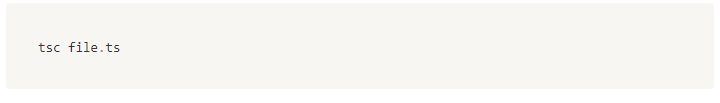
\includegraphics[width=15cm]{assets/tsbuild}\newline


		Cette commande nous créara un fichier JS du nom de file.js

	\end{frame}

	\begin{frame}
		\frametitle{TypeScript}

		Typescript ajoute la déclaration de variable: \newline \newline


		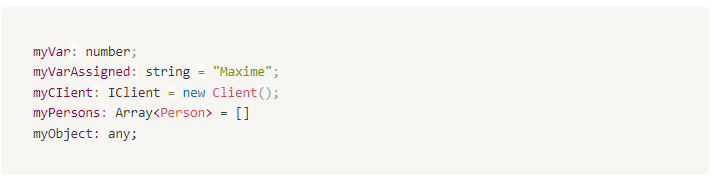
\includegraphics[width=15cm]{assets/tsvariable}\newline


	\end{frame}

	\begin{frame}
		\frametitle{TypeScript}

		Typescript ajoute la déclaration de variable: \newline \newline

		\centering
		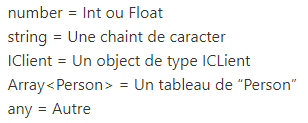
\includegraphics[width=7cm]{assets/tsvariable2}\newline


	\end{frame}


	\begin{frame}
		\frametitle{TypeScript}

		Activité : \newline \newline

		- Installer de quoi compile TypeScript avec cette comande \newline \newline

		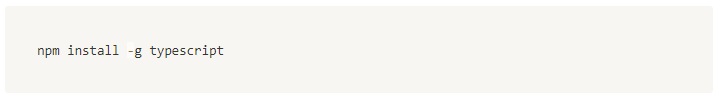
\includegraphics[width=16cm]{assets/tsInstall}\newline


	\end{frame}

	\begin{frame}
		\frametitle{TypeScript}

		Activité : \newline \newline




	\end{frame}

	\begin{frame}
		\frametitle{TypeScript}

		Activité : \newline \newline




	\end{frame}

%%%%%%%% Premier pas avec Angular

	\begin{frame}
		\frametitle{Premier pas avec Angular}

		Angular-CLI :  \newline \newline

		\centering
		Cette application vas installer tout ce qu’on a besoin \newline en une seul ligne de commande  \newline \newline

		et avec cette même outils on vas pouvoir piloté certaine fonctionnalité d’angular directement en ligne de command  \newline \newline

		\begin{block}{Information}
			Ce n'est pas la seul méthode pour démarré un projet Angular, mais bien la plus connue
		\end{block}

	\end{frame}


	\begin{frame}
		\frametitle{Premier pas avec Angular}

		Activité : \newline \newline

		- Installer Angular-CLI  \newline \newline

		Grace à NPM :  \newline \newline

		npm install -g @angular/cli


	\end{frame}

	\begin{frame}
		\frametitle{Premier pas avec Angular}

		Activité : \newline \newline

		- Verifier l'installation de Angular-CLI  \newline \newline

		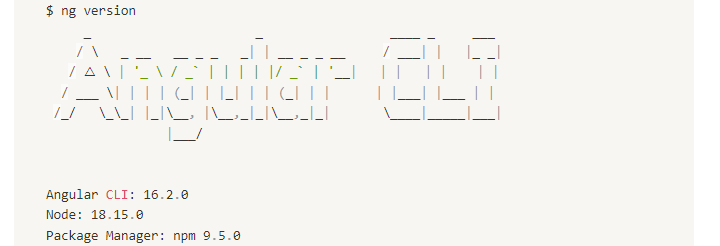
\includegraphics[width=16cm]{assets/angularCLInstall} \newline

		\begin{block}{Information}
			Toute les commande d'angular-cli ce feront avec le prefix NG
		\end{block}

	\end{frame}

	\begin{frame}
		\frametitle{Premier pas avec Angular}

		Nous alons generez notre premier projet Angular \newline \newline

		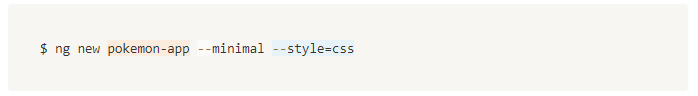
\includegraphics[width=16cm]{assets/angularsetup} \newline \newline

		Le nom du projet = pokemon-app \newline
		le type de ficher de style = css

	\end{frame}


	\begin{frame}
		\frametitle{Premier pas avec Angular}

		Activité : \newline
		Créer notre projet Angular \newline \newline

		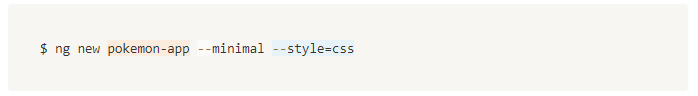
\includegraphics[width=17cm]{assets/angularsetup} \newline \newline

	\end{frame}

	\begin{frame}
		\frametitle{Premier pas avec Angular}

		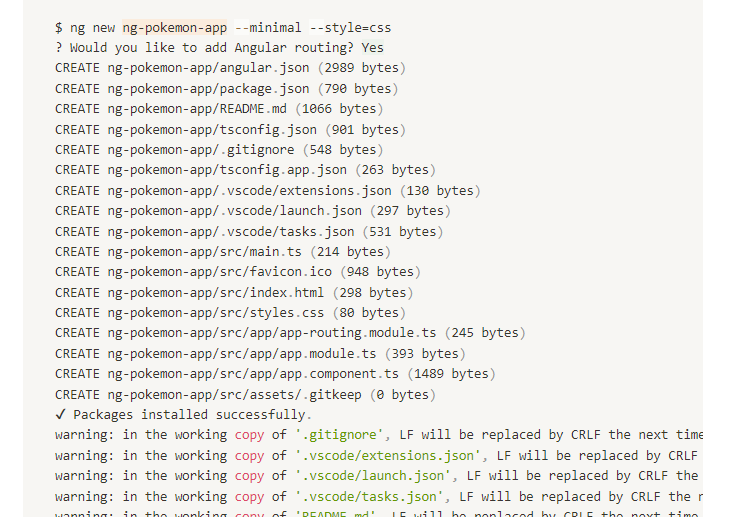
\includegraphics[width=15cm]{assets/angularsetup2} \newline \newline

	\end{frame}

	\begin{frame}
		\frametitle{Premier pas avec Angular}

		Que fait "Ng New" \newline \newline

		- Il créer tout le socle d'Augular\newline
		- Il installe toute les dépendance d'Angular (Il effectue des simple NPM INSTALL)\newline
		- Il initialise un .git \newline
		- Setup des confugurations pour des IDE\newline

	\end{frame}

	\begin{frame}
		\frametitle{Premier pas avec Angular}

		\centering
		Présentation du socle \newline \newline

	\end{frame}

	\begin{frame}
		\frametitle{Premier pas avec Angular}

		Lancé Angular : \newline \newline

		\centering
		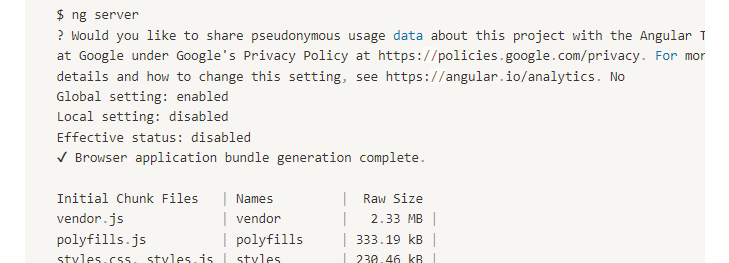
\includegraphics[width=15cm]{assets/ngserve} \newline

	\end{frame}

	\begin{frame}
		\frametitle{Premier pas avec Angular}

		\centering
		Inspection premier composant \newline \newline

	\end{frame}

	\begin{frame}
		\frametitle{Premier pas avec Angular}

		\centering
		Inspection du module racine \newline \newline

	\end{frame}

	\begin{frame}
		\frametitle{Premier pas avec Angular}

		\centering
		Configuration TypeScript \newline \newline


		\centering
		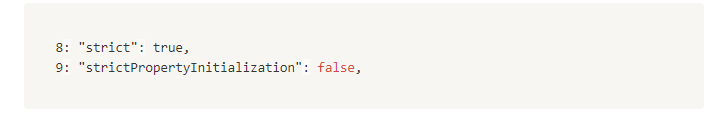
\includegraphics[width=11cm]{assets/tsConfig} \newline

	\end{frame}

%%%%%%%% Composant

	\begin{frame}
		\frametitle{Composants}

		Quest-ce qu'un composants ? : \newline \newline

		Un composants est une parti de l'écran \newline \newline

		Cette portion de l’écran qu’on vas controller,\newline on appel ça une vue  (ligne 5) \newline \newline

		cette vue est deffini dans le template et ça peut-etre beaucoup chose \newline \newline

		Donc un composant est une class + une vue
	\end{frame}

	\begin{frame}
		\frametitle{Composants}

		Quest-ce qu'un composants ? : \newline \newline

		le template (la vue) c'est le rendu pour les utilisateurs

		\centering
		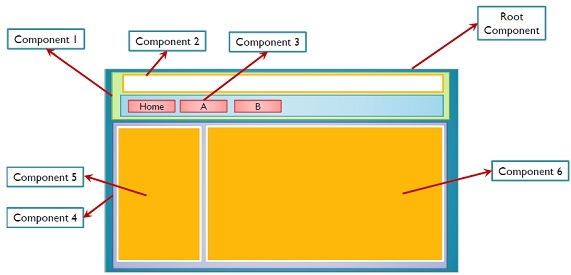
\includegraphics[width=11cm]{assets/composant} \newline


	\end{frame}

	\begin{frame}
		\frametitle{Composants}

		Première variable : \newline \newline

		\centering
		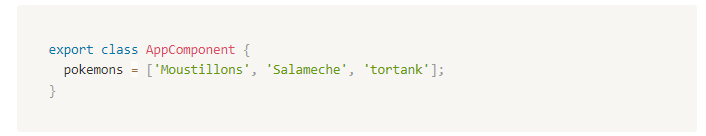
\includegraphics[width=11cm]{assets/tableauComposant} \newline

	\end{frame}

	\begin{frame}
		\frametitle{Composants}

		Activité : \newline \newline

		Afficher un pokémon dans votre template !

	\end{frame}

	\begin{frame}
		\frametitle{Composants}

		Affichage de notre première variable : \newline \newline

		\centering
		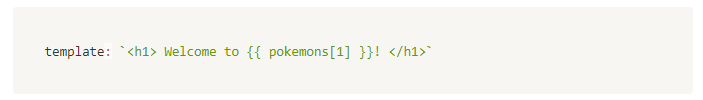
\includegraphics[width=11cm]{assets/templateComposant} \newline

	\end{frame}


	\begin{frame}
		\frametitle{Composants}

		Activité : \newline \newline


	\end{frame}

	\begin{frame}
		\frametitle{Composants}

		Activité : \newline \newline


	\end{frame}

	\begin{frame}
		\frametitle{Composants}

		Cycle de vie : \newline

		\centering
		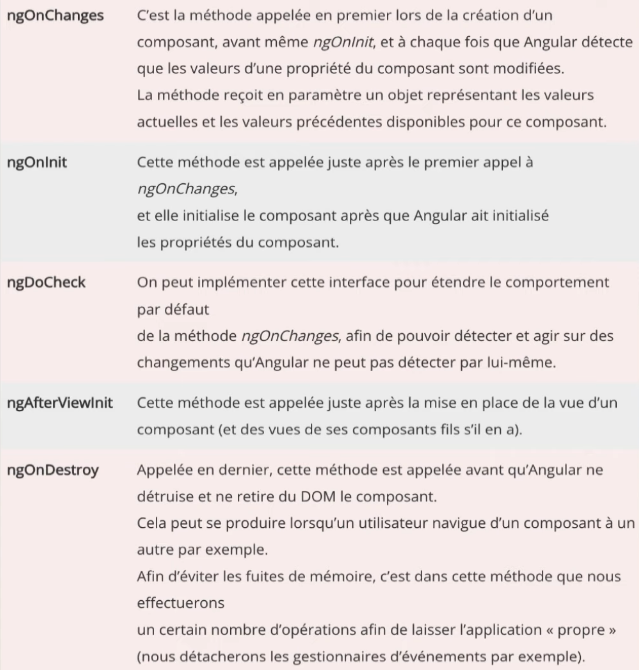
\includegraphics[width=7cm]{assets/vie} \newline


	\end{frame}

	\begin{frame}
		\frametitle{Composants}

		NgOnInit : \newline \newline

		On vas en chargant ce composont \newline vouloir afficher le tableau pokemon dans un console.log \newline \newline

		On vas devoir importé la fonctionnalité nessesaire  \newline \newline


	\end{frame}

	\begin{frame}
		\frametitle{Composants}

		NgOnInit : \newline \newline


		\centering
		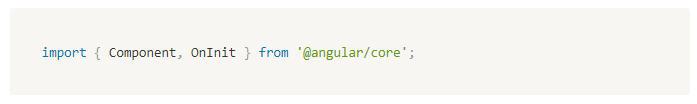
\includegraphics[width=11cm]{assets/ngoninit1} \newline


	\end{frame}

	\begin{frame}
		\frametitle{Composants}

		NgOnInit : \newline \newline


		\centering
		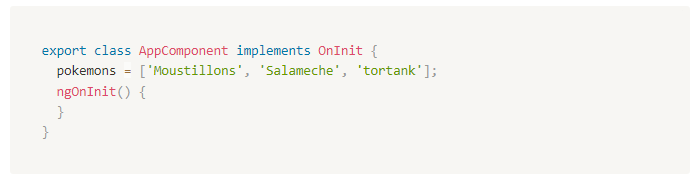
\includegraphics[width=11cm]{assets/ngoninit2} \newline


	\end{frame}

	\begin{frame}
		\frametitle{Composants}

		\centering
		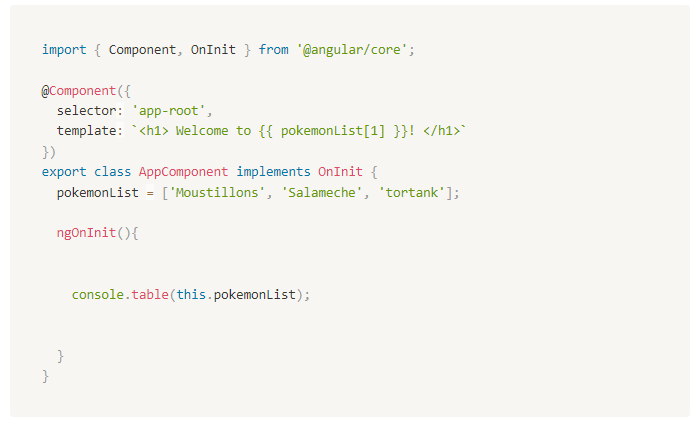
\includegraphics[width=12cm]{assets/consoleTable} \newline


	\end{frame}

	\begin{frame}
		\frametitle{Composants}

		Activité : \newline \newline


	\end{frame}

	\begin{frame}
		\frametitle{Composants}

		Interaction Utilisateur : \newline \newline

		On vas simplement créer une function qui affiche notre pokémon dans la console \newline \newline

		Une fois cette fonctionne créer, on vera dans le template comment activé cette fonction


	\end{frame}

	\begin{frame}
		\frametitle{Composants}

		Interaction Utilisateur : \newline \newline


		\centering
		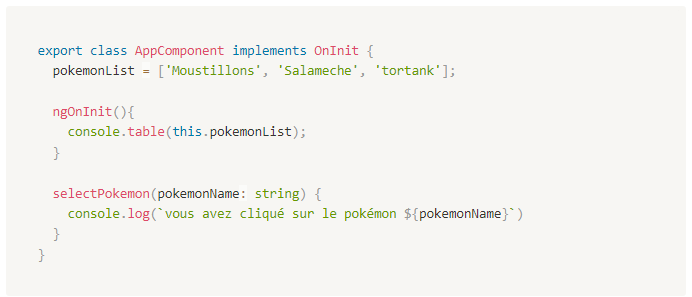
\includegraphics[width=12cm]{assets/userInt} \newline


	\end{frame}

	\begin{frame}
		\frametitle{Composants}

		Interaction Utilisateur : \newline \newline

		Pour tester cette fonction sans le template, on vas lancer la fonction au lancement du composant

		\centering
		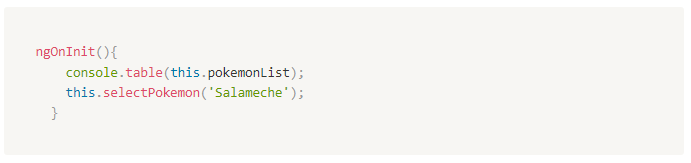
\includegraphics[width=12cm]{assets/userInt2} \newline


	\end{frame}

	\begin{frame}
		\frametitle{Composants}

		Activité : \newline \newline


	\end{frame}

	\begin{frame}
		\frametitle{Composants}

		Activité : \newline \newline


	\end{frame}

	\begin{frame}
		\frametitle{Composants}

		Gerez de la donnée : \newline \newline

		nous allons créer deux fichier \newline \newline

		- ./src/app/pokemons.ts \newline
		- ./src/app/mock-pokemons-list.ts \newline \newline

		Le premier est un model (Class D'Object en php) \newline \newline

		Le Deuxième un tableau basé sur le model qui contient de la donnée

	\end{frame}

	\begin{frame}
		\frametitle{Composants}

		Activité : \newline \newline

		- Afficher en titre "Liste de pokémon" \newline
		- Recupéré dans la pokemonList toute les donnée du mock \newline
		- Dans la fonction selectPokemon recupéré tout un model pokémon plutot qu'un String \newline

	\end{frame}

	\begin{frame}
		\frametitle{Composants}

		Activité : \newline \newline


	\end{frame}

%%%%%%%% Template
	\begin{frame}
		\frametitle{Template}

		Laisser la vue au même endroit que la logique \newline
		C'est absolument pas \alert{recommander} \newline \newline

		Alors dans notre composant on vas changer ça, \newline en créant un ficher appart\newline \newline

	\end{frame}

	\begin{frame}
		\frametitle{Template}

		On vas créer un fichier : \newline
		- ./src/app/app.component.html \newline \newline

		et modifier le composant : \newline


		\centering
		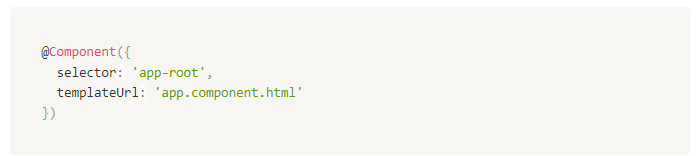
\includegraphics[width=12cm]{assets/templateAsset} \newline

	\end{frame}

	\begin{frame}
		\frametitle{Template}

		Dans app.component.html : \newline

		\centering
		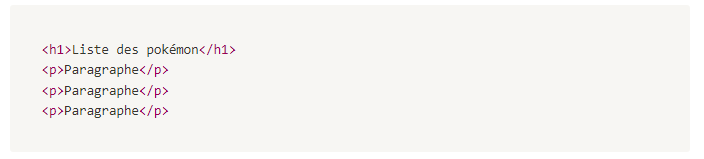
\includegraphics[width=14cm]{assets/templateHtml} \newline

	\end{frame}

	\begin{frame}
		\frametitle{Template}

		On peut constater que la vue ce charge bien par le biais de notre fichier html \newline \newline

		Et il y a bien toujours notre logique dans la console JavaScript  \newline \newline

		Donc maintenant on a fichier \alert{Logique} (Composant) et un fichier \alert{Graphique} (Template) \newline \newline

		c’est ce systeme qu’on vas utiliser tout au long du developpement Angular

	\end{frame}

	\begin{frame}
		\frametitle{Template}

		Activité : \newline \newline


	\end{frame}

	\begin{frame}
		\frametitle{Template}

		Activité : \newline \newline


	\end{frame}

	\begin{frame}
		\frametitle{Template}

		L'interpolation : \newline \newline

		Nous avons actuellement un fichier HTML \alert{static} \newline \newline

		Et nous voulons le rendre \alert{dynamique} \newline \newline

		On vas utiliser la syntaxe d’interpolation


	\end{frame}

	\begin{frame}
		\frametitle{Template}

		L'interpolation : \newline \newline


		\centering
		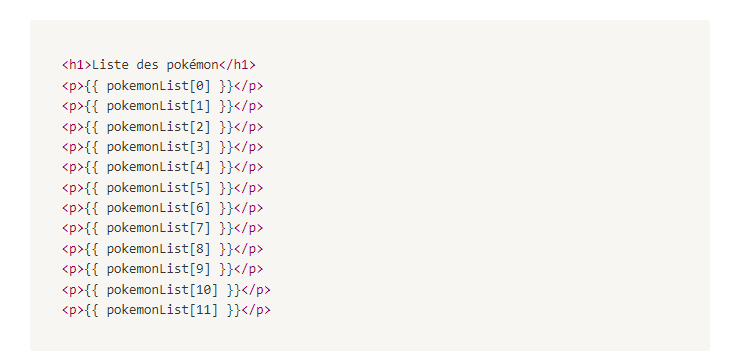
\includegraphics[width=14cm]{assets/inter} \newline


	\end{frame}

	\begin{frame}
		\frametitle{Template}

		L'interpolation : \newline \newline


		\centering
		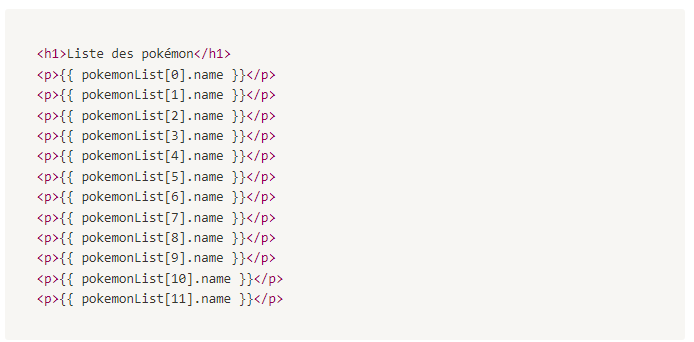
\includegraphics[width=14cm]{assets/inter2} \newline


	\end{frame}


\end{document}